% =============================================================================
% parallel_concepts_diagrams.tex
% Analysis Report – Diagrams & Descriptions
% "How Parallel Programming Concepts Were Applied"
%
% EC7207 / EE7218  High Performance Computing  –  Group 11
% Topic: Pearson Correlation-Based Recommendation System
%
% Compile:
%   pdflatex parallel_concepts_diagrams.tex   (run twice for correct spacing)
% =============================================================================
\documentclass[12pt,a4paper]{article}

\usepackage[margin=2.2cm]{geometry}
\setlength{\headheight}{14pt}
\usepackage{tikz}
\usetikzlibrary{arrows.meta, shapes.geometric, positioning, fit,
                decorations.pathreplacing, matrix, calc, backgrounds,
                patterns, shadows.blur}
% Allow \\ line breaks inside every node (centered multi-line text).
\tikzset{every node/.append style={align=center}}
\usepackage{amsmath}
\usepackage{booktabs}
\usepackage{xcolor}
\usepackage{colortbl}   % \rowcolor in comparison tables
\usepackage{enumitem}
\usepackage{fancyhdr}
\usepackage{titlesec}
\usepackage{mdframed}
\usepackage{array}
\usepackage{multicol}
\usepackage{caption}

% ── Colour palette ────────────────────────────────────────────────────────────
\definecolor{serialcol}{RGB}{70,130,180}      % steel blue
\definecolor{ompcol}{RGB}{34,139,34}          % forest green
\definecolor{pthcol}{RGB}{184,134,11}         % dark goldenrod
\definecolor{mpicol}{RGB}{178,34,34}          % firebrick
\definecolor{cudacol}{RGB}{118,0,163}         % purple
\definecolor{hybcol}{RGB}{210,90,0}           % burnt orange
\definecolor{lightgray2}{RGB}{245,245,245}
\definecolor{darkgray2}{RGB}{80,80,80}

% ── Page style ────────────────────────────────────────────────────────────────
\pagestyle{fancy}
\fancyhf{}
\lhead{\small EC7207/EE7218 HPC — Group 11}
\rhead{\small Parallel Programming Concept Diagrams}
\cfoot{\small\thepage}

\titleformat{\section}{\large\bfseries\color{darkgray2}}{}{0em}{}[\vspace{-4pt}\rule{\linewidth}{0.8pt}]
\titleformat{\subsection}{\normalsize\bfseries}{}{0em}{}

% ── Description box style ─────────────────────────────────────────────────────
\mdfdefinestyle{descbox}{
  linewidth=1pt, linecolor=darkgray2!50,
  backgroundcolor=lightgray2,
  innerleftmargin=10pt, innerrightmargin=10pt,
  innertopmargin=8pt, innerbottommargin=8pt,
  skipabove=6pt, skipbelow=6pt
}

% =============================================================================
\begin{document}
% =============================================================================

% ── Title ─────────────────────────────────────────────────────────────────────
\begin{center}
{\LARGE\bfseries Parallel Programming Concepts Applied}\\[0.4em]
{\large\bfseries to the Pearson Correlation Recommender System}\\[0.3em]
{\normalsize EC7207/EE7218 High Performance Computing \ $\bullet$\  Group 11}
\end{center}
\vspace{0.5em}
\hrule height 1.5pt
\vspace{1em}

% ── Intro paragraph ───────────────────────────────────────────────────────────
\noindent
This section presents diagrams and descriptions that illustrate how each of the
five parallel programming paradigms — \textbf{OpenMP}, \textbf{POSIX Threads
(Pthreads)}, \textbf{MPI}, \textbf{CUDA}, and \textbf{Hybrid MPI+OpenMP} — was
applied to accelerate a User-Based Collaborative Filtering recommender system.
The system computes Pearson Correlation similarity between 1\,000 users over
1\,000 items, predicts unseen ratings, and evaluates Mean Absolute Error (MAE).

\vspace{0.5em}

% =============================================================================
\section{System Overview: The 5-Phase Algorithm Pipeline}
% =============================================================================

\subsection*{Diagram 1 — Algorithm Flow and Parallelisation Targets}

\begin{center}
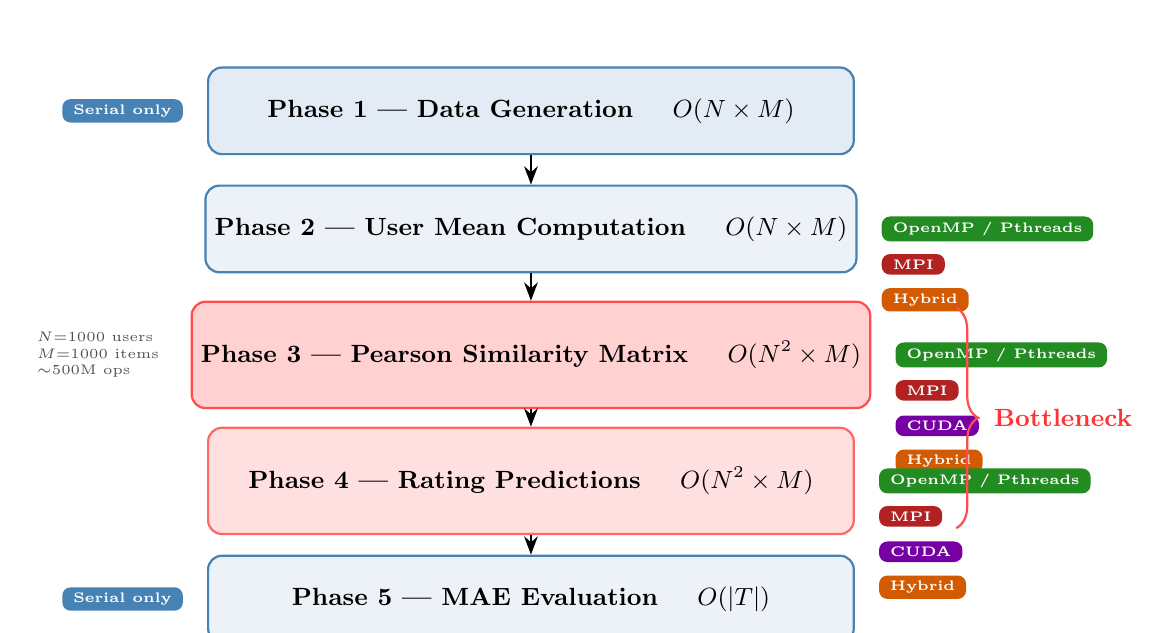
\begin{tikzpicture}[
  phase/.style={rectangle, rounded corners=5pt, minimum width=8.2cm,
                minimum height=1.1cm, text centered, font=\small\bfseries,
                draw, thick},
  arrow/.style={-Stealth, thick},
  badge/.style={rectangle, rounded corners=3pt, font=\tiny\bfseries,
                inner xsep=4pt, inner ysep=2pt, text=white}
]

% Phase boxes
\node[phase, fill=serialcol!15, draw=serialcol]
      (p1) at (0,0)
      {Phase 1 — Data Generation \quad $O(N \times M)$};

\node[phase, fill=serialcol!10, draw=serialcol]
      (p2) at (0,-1.5)
      {Phase 2 — User Mean Computation \quad $O(N \times M)$};

\node[phase, fill=red!18, draw=red!70, minimum width=8.2cm, minimum height=1.35cm]
      (p3) at (0,-3.1)
      {Phase 3 — Pearson Similarity Matrix \quad $O(N^2 \times M)$};

\node[phase, fill=red!12, draw=red!60, minimum width=8.2cm, minimum height=1.35cm]
      (p4) at (0,-4.7)
      {Phase 4 — Rating Predictions \quad $O(N^2 \times M)$};

\node[phase, fill=serialcol!10, draw=serialcol]
      (p5) at (0,-6.2)
      {Phase 5 — MAE Evaluation \quad $O(|T|)$};

% Arrows
\foreach \a/\b in {p1/p2, p2/p3, p3/p4, p4/p5}
  \draw[arrow] (\a) -- (\b);

% Parallel badges on the right
\node[badge, fill=ompcol, right=0.3cm of p2.east, anchor=west]  {OpenMP / Pthreads};
\node[badge, fill=mpicol,  right=0.3cm of p2.east, anchor=west, yshift=-0.45cm]  {MPI};
\node[badge, fill=hybcol,  right=0.3cm of p2.east, anchor=west, yshift=-0.9cm]  {Hybrid};

\node[badge, fill=ompcol, right=0.3cm of p3.east, anchor=west]  {OpenMP / Pthreads};
\node[badge, fill=mpicol,  right=0.3cm of p3.east, anchor=west, yshift=-0.45cm]  {MPI};
\node[badge, fill=cudacol, right=0.3cm of p3.east, anchor=west, yshift=-0.9cm]  {CUDA};
\node[badge, fill=hybcol,  right=0.3cm of p3.east, anchor=west, yshift=-1.35cm] {Hybrid};

\node[badge, fill=ompcol, right=0.3cm of p4.east, anchor=west]  {OpenMP / Pthreads};
\node[badge, fill=mpicol,  right=0.3cm of p4.east, anchor=west, yshift=-0.45cm]  {MPI};
\node[badge, fill=cudacol, right=0.3cm of p4.east, anchor=west, yshift=-0.9cm]  {CUDA};
\node[badge, fill=hybcol,  right=0.3cm of p4.east, anchor=west, yshift=-1.35cm] {Hybrid};

% Serial label on the left
\node[badge, fill=serialcol, left=0.3cm of p1.west, anchor=east] {Serial only};
\node[badge, fill=serialcol, left=0.3cm of p5.west, anchor=east] {Serial only};

% Bottleneck brace
\draw[decorate, decoration={brace,amplitude=8pt}, thick, red!70]
     (5.4,-2.5) -- (5.4,-5.3)
     node[midway, right=10pt, font=\small\bfseries, red!80] {Bottleneck};

% Complexity annotation
\node[font=\tiny\color{darkgray2}, align=left] at (-5.5,-3.1)
      {$N{=}1000$ users\\ $M{=}1000$ items\\ ${\sim}500$M ops};

\end{tikzpicture}
\end{center}

\begin{mdframed}[style=descbox]
\textbf{Description.} The recommender system executes in five sequential
phases.  Phases~1 and~5 are inherently serial: data generation uses a fixed
random seed (\texttt{SEED=42}) to ensure identical inputs across all versions,
and MAE evaluation is fast ($O(|T|)$) and not a bottleneck.  Phases~2--4 are
parallelised.  The dominant cost lies in Phases~3 and~4, each of $O(N^2
\times M)$ complexity — approximately 500 million floating-point operations
for a $1000 \times 1000$ matrix.  These are the targets for acceleration with
OpenMP, Pthreads, MPI, CUDA, and Hybrid parallelism.
\end{mdframed}

\newpage

% =============================================================================
\section{Data Structure: Ratings Matrix and Row Partitioning}
% =============================================================================

\subsection*{Diagram 2 — Flat Row-Major Storage and Work Division}

\begin{center}
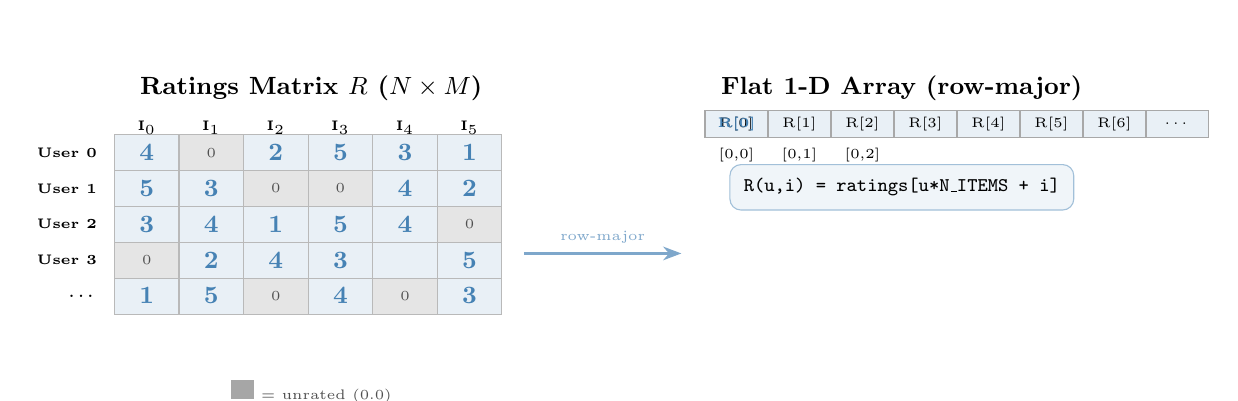
\begin{tikzpicture}[x=1cm, y=0.7cm]

% ── Logical matrix (left) ────────────────────────────────────────────────────
\node[font=\small\bfseries] at (2.5,1.5) {Ratings Matrix $R$ \small($N \times M$)};
\foreach \row in {0,...,4} {
  \foreach \col in {0,...,5} {
    \pgfmathsetmacro\val{int(random(0,5))}
    \pgfmathsetmacro\isgray{(\col==2 && \row==1) || (\col==4 && \row==3)
                          || (\col==1 && \row==0) || (\col==5 && \row==2)
                          || (\col==0 && \row==4) || (\col==3 && \row==1)}
    \ifnum\row=0
      \ifnum\col=1 \def\fillcol{white}\else\def\fillcol{serialcol!12}\fi
    \else
      \def\fillcol{serialcol!12}
    \fi
    \draw[fill=\fillcol, draw=darkgray2!40]
         (\col*0.82, -\row*0.65) rectangle (\col*0.82+0.82, -\row*0.65+0.65);
  }
}
% Zero entries (unrated)
\foreach \r/\c in {0/1, 1/2, 1/3, 2/5, 3/0, 4/2, 4/4} {
  \draw[fill=gray!20, draw=darkgray2!40]
       (\c*0.82, -\r*0.65) rectangle (\c*0.82+0.82, -\r*0.65+0.65);
  \node[font=\tiny\color{darkgray2}] at (\c*0.82+0.41, -\r*0.65+0.33) {0};
}
% Non-zero values
\foreach \r/\c/\v in {0/0/4, 0/2/2, 0/3/5, 0/4/3, 0/5/1,
                       1/0/5, 1/1/3, 1/4/4, 1/5/2,
                       2/0/3, 2/1/4, 2/2/1, 2/3/5, 2/4/4,
                       3/1/2, 3/2/4, 3/3/3, 3/5/5,
                       4/0/1, 4/1/5, 4/3/4, 4/5/3} {
  \node[font=\small\bfseries, serialcol] at (\c*0.82+0.41, -\r*0.65+0.33) {\v};
}
% Row labels
\foreach \r/\lbl in {0/User 0, 1/User 1, 2/User 2, 3/User 3, 4/\ldots} {
  \node[font=\tiny\bfseries, anchor=east] at (-0.1, -\r*0.65+0.33) {\lbl};
}
% Column labels
\foreach \c/\lbl in {0/I$_0$, 1/I$_1$, 2/I$_2$, 3/I$_3$, 4/I$_4$, 5/I$_5$} {
  \node[font=\tiny\bfseries] at (\c*0.82+0.41, 0.78) {\lbl};
}
% Zero legend
\node[font=\tiny, darkgray2, align=left] at (2.5,-4.0)
      {\textcolor{gray!70}{\rule{0.3cm}{0.25cm}} = unrated (0.0)};

% ── Flat array (right) ───────────────────────────────────────────────────────
\node[font=\small\bfseries] at (10,1.5) {Flat 1-D Array (row-major)};
\foreach \i in {0,...,7} {
  \draw[fill=serialcol!12, draw=darkgray2!50]
       (7.5+\i*0.8, 0.6) rectangle (7.5+\i*0.8+0.8, 1.1);
  \node[font=\tiny] at (7.9+\i*0.8, 0.85)
        {\ifnum\i=7\ldots\else R[\i]\fi};
}
\node[font=\tiny\bfseries,serialcol] at (7.9,0.85) {R[0]};
\node[font=\tiny, anchor=north] at (7.9, 0.58) {\tiny[0,0]};
\node[font=\tiny, anchor=north] at (8.7, 0.58) {\tiny[0,1]};
\node[font=\tiny, anchor=north] at (9.5, 0.58) {\tiny[0,2]};

% Macro annotation
\node[font=\scriptsize, align=center, draw=serialcol!50, rounded corners,
      fill=serialcol!8, inner sep=5pt] at (10,-0.3)
      {\texttt{R(u,i) = ratings[u*N\_ITEMS + i]}};

% Arrow from matrix to flat
\draw[-Stealth, thick, serialcol!70] (5.2,-1.5) -- (7.2,-1.5)
      node[midway,above,font=\tiny]{row-major};

\end{tikzpicture}
\end{center}

\begin{mdframed}[style=descbox]
\textbf{Description.} The ratings matrix $R$ ($N_{\text{users}} \times
M_{\text{items}}$) is stored as a flat 1-D array in row-major order.
Entry $R[u,i]$ is accessed via the macro \texttt{R(u,i) = ratings[u*N\_ITEMS + i]}.
A value of $0.0$ indicates an unrated cell.  This storage layout enables a
single \texttt{calloc} call per matrix, maximises CPU cache utilisation during
row scans, and simplifies inter-rank communication in MPI
(\texttt{MPI\_Allgatherv} sends contiguous row blocks).
The same layout is used for the $N \times N$ similarity matrix
(\texttt{sim\_matrix}) and the predictions matrix.
\end{mdframed}

\newpage

% =============================================================================
\section{OpenMP — Shared-Memory Fork-Join Parallelism}
% =============================================================================

\subsection*{Diagram 3 — OpenMP Applied to the Similarity Phase}

\begin{center}
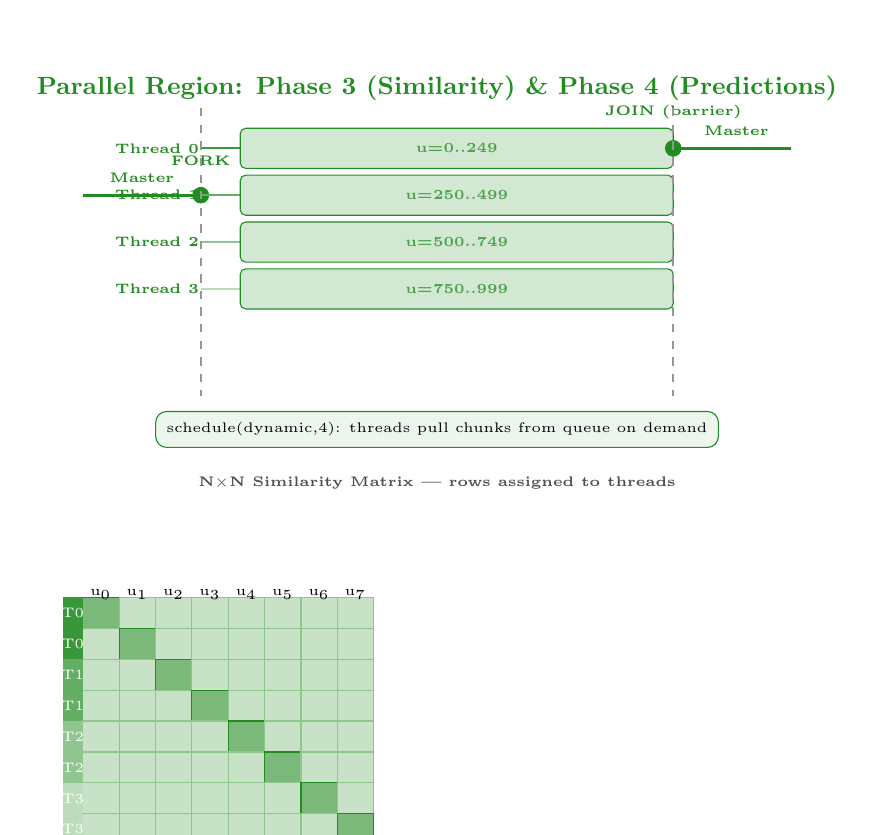
\begin{tikzpicture}[x=1cm,y=0.85cm]

% ── Fork-Join bar ─────────────────────────────────────────────────────────────
\draw[ompcol, very thick] (0,0) -- (1.5,0);
\node[font=\tiny\bfseries, ompcol, above] at (0.75,0.05) {Master};

% Fork point
\fill[ompcol] (1.5,0) circle (3pt);
\node[font=\tiny, ompcol, above] at (1.5,0.3) {\textbf{FORK}};

% Thread lanes
\foreach \t/\col in {0/ompcol!90, 1/ompcol!70, 2/ompcol!50, 3/ompcol!30} {
  \draw[\col, thick] (1.5, -\t*0.7+0.7) -- (7.5, -\t*0.7+0.7);
}
% Thread labels
\foreach \t in {0,1,2,3} {
  \node[font=\tiny\bfseries, ompcol, left] at (1.6, -\t*0.7+0.7)
        {Thread \t};
}

% Work blocks on each thread lane
\foreach \t/\s/\e/\lbl in {
  0/2.0/3.8/u=0..249,
  1/2.0/5.2/u=250..499,
  2/2.0/6.2/u=500..749,
  3/2.0/7.5/u=750..999}
{
  \draw[fill=ompcol!20, draw=ompcol, rounded corners=2pt]
       (\s, -\t*0.7+0.4) rectangle (7.5, -\t*0.7+1.0);
  \node[font=\tiny\bfseries, ompcol!80] at ({(\s+7.5)/2}, -\t*0.7+0.7) {\lbl};
}

% Dynamic queue arrow
\node[draw=ompcol, rounded corners, font=\tiny, fill=ompcol!8,
      inner sep=4pt] at (4.5,-3.5)
      {schedule(dynamic,4): threads pull chunks from queue on demand};

% Join point
\fill[ompcol] (7.5,0.7) circle (3pt);
\draw[ompcol, very thick] (7.5,0.7) -- (9,0.7);
\node[font=\tiny\bfseries, ompcol, above] at (7.5,1.0) {\textbf{JOIN (barrier)}};
\node[font=\tiny\bfseries, ompcol, above] at (8.3,0.75) {Master};

% Vertical barrier lines
\draw[dashed, darkgray2!60, thick] (1.5,1.3) -- (1.5,-3.0);
\draw[dashed, darkgray2!60, thick] (7.5,1.3) -- (7.5,-3.0);

% Phases label
\node[font=\small\bfseries, ompcol] at (4.5,1.6)
      {Parallel Region: Phase~3 (Similarity) \& Phase~4 (Predictions)};

% Similarity matrix visual below
\node[font=\tiny\bfseries, darkgray2] at (4.5,-4.3)
      {N$\times$N Similarity Matrix — rows assigned to threads};
\begin{scope}[yshift=-5.5cm, xscale=0.42, yscale=0.42]
  \foreach \r in {0,...,7} {
    \foreach \c in {0,...,7} {
      \pgfmathsetmacro\tid{int(\r/2)}
      \pgfmathparse{\c > \r ? 1 : 0}
      \ifnum\c>\r
        \draw[fill=ompcol!25,draw=ompcol!50]
             (\c*1.1,-\r*1.1) rectangle (\c*1.1+1.1,-\r*1.1+1.1);
      \else
        \ifnum\c=\r
          \draw[fill=ompcol!60,draw=ompcol]
               (\c*1.1,-\r*1.1) rectangle (\c*1.1+1.1,-\r*1.1+1.1);
        \else
          \draw[fill=ompcol!25,draw=ompcol!50]
               (\c*1.1,-\r*1.1) rectangle (\c*1.1+1.1,-\r*1.1+1.1);
        \fi
      \fi
    }
    % Thread colour bands on left
    \pgfmathsetmacro\tidx{int(\r/2)}
    \draw[fill=ompcol!\the\numexpr 90-\tidx*20\relax, draw=none]
         (-0.6,-\r*1.1) rectangle (-0.0,-\r*1.1+1.1);
    \node[font=\tiny, white] at (-0.3,-\r*1.1+0.55) {T\tidx};
  }
  % Labels
  \foreach \c in {0,...,7} {
    \node[font=\tiny] at (\c*1.1+0.55,1.2) {u$_\c$};
  }
\end{scope}

\end{tikzpicture}
\end{center}

\begin{mdframed}[style=descbox]
\textbf{Description.}  OpenMP parallelises Phases~2--5 using compiler
directives (\texttt{\#pragma omp}).  In Phase~3 (similarity), each thread
receives a dynamic chunk of outer-loop iterations $u$ and computes Pearson
correlations for all $v > u$ in that chunk, writing to disjoint rows of
\texttt{sim\_matrix[]}.  \texttt{schedule(dynamic,4)} is used because the
inner loop shrinks as $u$ increases — thread 0 processes far more pairs
than thread 3, so static equal-chunk assignment would cause severe load
imbalance; dynamic scheduling lets idle threads pull new chunks from a
shared queue.  In Phase~4 (predictions), each thread allocates its own
private neighbour buffer (\texttt{malloc} inside \texttt{\#pragma omp
parallel}) to avoid any shared-state race.  An implicit OpenMP barrier at
the end of each parallel region ensures phase ordering.  The serial
fraction (Phase~1 data generation, Phase~5 MAE output) is $\approx 2$--$3\%$,
limiting maximum speedup to $\approx 35$--$50\times$ by Amdahl's Law.
\end{mdframed}

\newpage

% =============================================================================
\section{Pthreads — Manual POSIX Thread Management}
% =============================================================================

\subsection*{Diagram 4 — Pthreads Lifecycle and Work Partitioning}

\begin{center}
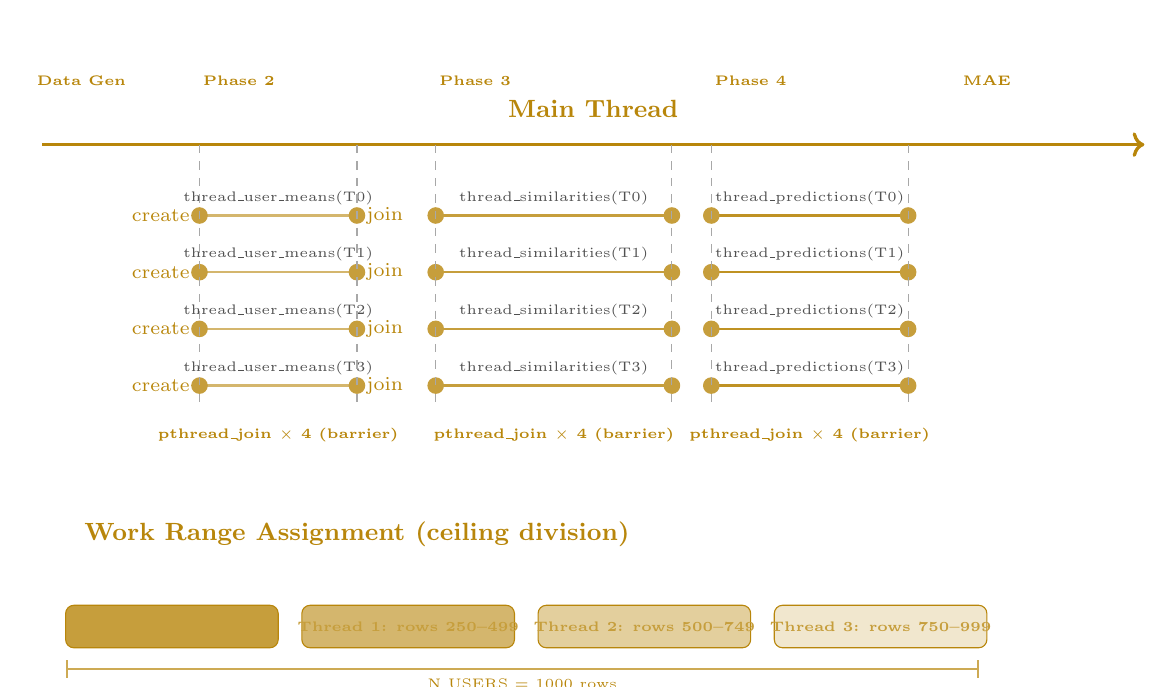
\begin{tikzpicture}[x=1cm,y=0.9cm]

% ── Main thread timeline ──────────────────────────────────────────────────────
\draw[pthcol, very thick, ->] (0,0) -- (14,0);
\node[font=\small\bfseries, pthcol] at (7,0.5) {Main Thread};

% ── Phase labels on timeline ─────────────────────────────────────────────────
\foreach \x/\lbl in {0.5/Data Gen, 2.5/Phase 2, 5.5/Phase 3, 9/Phase 4, 12/MAE} {
  \node[font=\tiny\bfseries, pthcol, above] at (\x, 0.7) {\lbl};
}

% ── Thread create/join events ────────────────────────────────────────────────
% Phase 2 threads
\foreach \t/\y in {0/-1.0, 1/-1.8, 2/-2.6, 3/-3.4} {
  \draw[pthcol!60, thick] (2.0,\y) -- (4.0,\y);
  \fill[pthcol!80] (2.0,\y) circle (3pt)
                   (4.0,\y) circle (3pt);
  \node[font=\tiny, pthcol, left] at (2.0,\y) {\scriptsize create};
  \node[font=\tiny, pthcol, right] at (4.0,\y) {\scriptsize join};
  \node[font=\tiny, darkgray2] at (3.0,\y+0.25)
        {\tiny thread\_user\_means(T\t)};
}
\node[font=\tiny\bfseries, pthcol] at (3.0,-4.1) {pthread\_join $\times$ 4 (barrier)};

% Phase 3 threads
\foreach \t/\y in {0/-1.0, 1/-1.8, 2/-2.6, 3/-3.4} {
  \draw[pthcol!80, thick] (5.0,\y) -- (8.0,\y);
  \fill[pthcol!80] (5.0,\y) circle (3pt)
                   (8.0,\y) circle (3pt);
  \node[font=\tiny, darkgray2] at (6.5,\y+0.25)
        {\tiny thread\_similarities(T\t)};
}
\node[font=\tiny\bfseries, pthcol] at (6.5,-4.1) {pthread\_join $\times$ 4 (barrier)};

% Phase 4 threads
\foreach \t/\y in {0/-1.0, 1/-1.8, 2/-2.6, 3/-3.4} {
  \draw[pthcol!90, thick] (8.5,\y) -- (11.0,\y);
  \fill[pthcol!80] (8.5,\y) circle (3pt)
                   (11.0,\y) circle (3pt);
  \node[font=\tiny, darkgray2] at (9.75,\y+0.25)
        {\tiny thread\_predictions(T\t)};
}
\node[font=\tiny\bfseries, pthcol] at (9.75,-4.1) {pthread\_join $\times$ 4 (barrier)};

% Vertical create/join lines to main thread
\foreach \x in {2.0,4.0,5.0,8.0,8.5,11.0} {
  \draw[dashed, darkgray2!50] (\x,0) -- (\x,-3.7);
}

% Work range diagram
\node[font=\small\bfseries, pthcol] at (4.0,-5.5) {Work Range Assignment (ceiling division)};
\foreach \t/\s/\e/\col in {0/0/249/pthcol!80, 1/250/499/pthcol!60,
                             2/500/749/pthcol!40, 3/750/999/pthcol!20} {
  \draw[fill=\col, draw=pthcol, rounded corners=3pt]
       (0.3+\t*3.0,-6.5) rectangle (3.0+\t*3.0,-7.1);
  \node[font=\tiny\bfseries, pthcol!80] at (1.65+\t*3.0,-6.8)
        {Thread \t: rows \s--\e};
}
\draw[|-|, thick, pthcol!70] (0.3,-7.4) -- (11.9,-7.4);
\node[font=\tiny, pthcol, below] at (6.1,-7.4) {N\_USERS = 1000 rows};

\end{tikzpicture}
\end{center}

\begin{mdframed}[style=descbox]
\textbf{Description.}  The Pthreads version explicitly creates and joins
threads for each of the three parallel phases using a helper function
\texttt{run\_parallel()}.  A \texttt{ThreadArgs} struct
\texttt{\{tid, nthreads\}} is passed to each thread, from which the thread
independently computes its row range via ceiling division:
\texttt{chunk = (N\_USERS + nthreads - 1) / nthreads}.  Thread $t$ owns
rows $[t \times \text{chunk},\; (t+1) \times \text{chunk})$.  Since all
threads write to disjoint index ranges of \texttt{sim\_matrix[]} and
\texttt{predictions[]}, no mutex is required.  The private neighbour buffer
\texttt{nbrs[]} is allocated inside each thread function — each thread gets
its own heap allocation via \texttt{malloc()}, which is thread-safe.
\texttt{pthread\_join} after the last thread serves as a phase barrier,
guaranteeing that all similarity values are written before the prediction
phase reads them.
\end{mdframed}

\newpage

% =============================================================================
\section{MPI — Distributed-Memory Row Partitioning}
% =============================================================================

\subsection*{Diagram 5 — MPI Process Layout and Collective Communication}

\begin{center}
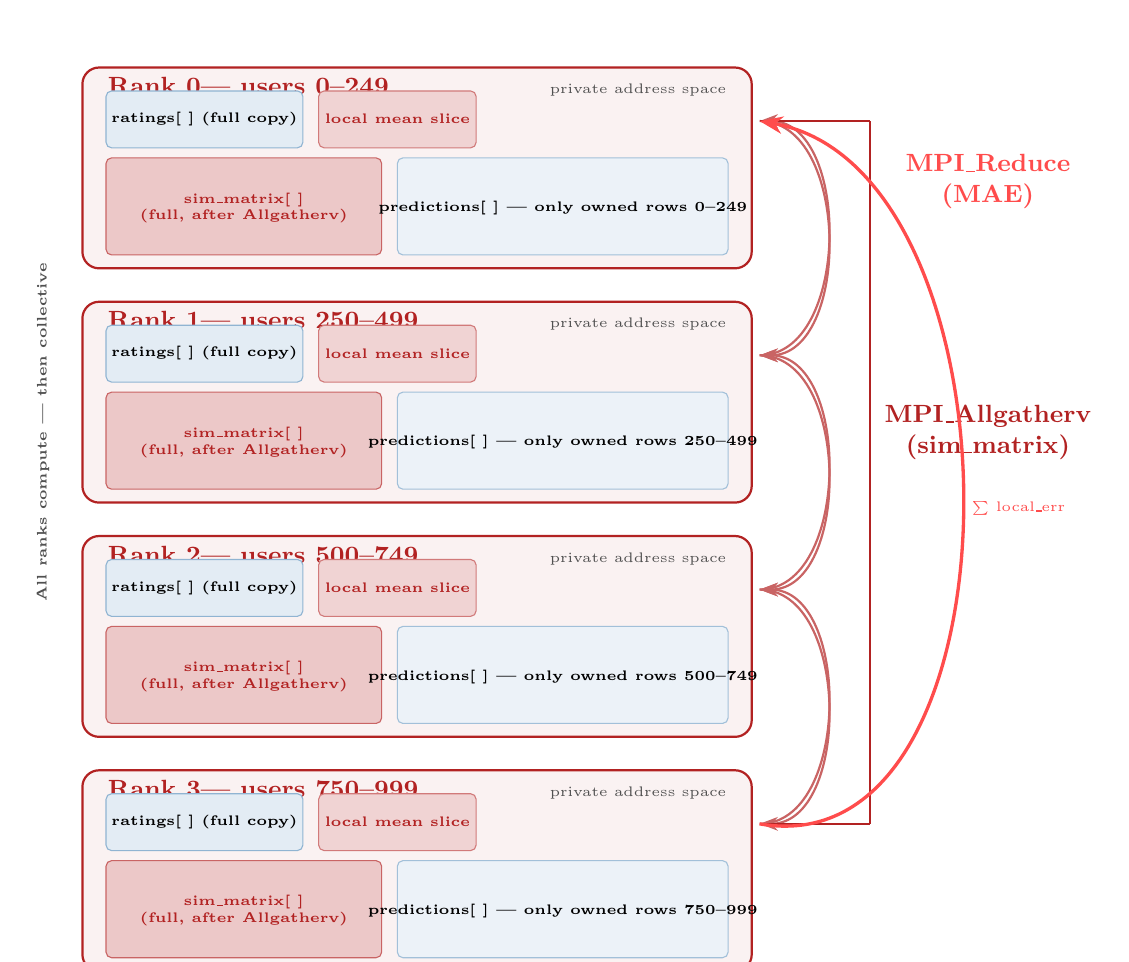
\begin{tikzpicture}[x=1cm,y=0.85cm]

% ── Four rank boxes ───────────────────────────────────────────────────────────
\foreach \r/\ypos/\label/\ufrom/\uto in {
    0/0/Rank 0/0/249,
    1/-3.5/Rank 1/250/499,
    2/-7.0/Rank 2/500/749,
    3/-10.5/Rank 3/750/999}
{
  % Rank container
  \draw[mpicol, thick, rounded corners=6pt, fill=mpicol!6]
       (0,\ypos-2.8) rectangle (8.5,\ypos+0.2);
  \node[font=\small\bfseries, mpicol, anchor=north west]
       at (0.2,\ypos+0.2) {\label — users \ufrom--\uto};

  % Private memory label
  \node[font=\tiny, darkgray2, anchor=north east]
       at (8.3,\ypos+0.1) {private address space};

  % Ratings block
  \draw[fill=serialcol!15, draw=serialcol!60, rounded corners=2pt]
       (0.3,\ypos-1.0) rectangle (2.8,\ypos-0.15);
  \node[font=\tiny\bfseries] at (1.55,\ypos-0.57) {ratings[ ] (full copy)};

  % Local mean block
  \draw[fill=mpicol!20, draw=mpicol!60, rounded corners=2pt]
       (3.0,\ypos-1.0) rectangle (5.0,\ypos-0.15);
  \node[font=\tiny\bfseries, mpicol] at (4.0,\ypos-0.57)
        {local mean slice};

  % Sim block
  \draw[fill=mpicol!25, draw=mpicol!70, rounded corners=2pt]
       (0.3,\ypos-2.6) rectangle (3.8,\ypos-1.15);
  \node[font=\tiny\bfseries, mpicol] at (2.05,\ypos-1.9)
        {sim\_matrix[ ]\\ (full, after Allgatherv)};

  % Pred block
  \draw[fill=serialcol!10, draw=serialcol!50, rounded corners=2pt]
       (4.0,\ypos-2.6) rectangle (8.2,\ypos-1.15);
  \node[font=\tiny\bfseries] at (6.1,\ypos-1.9)
        {predictions[ ] — only owned rows \ufrom--\uto};
}

% ── Allgatherv arrows (Phase 3) ──────────────────────────────────────────────
\node[font=\small\bfseries, mpicol] at (11.5,-5.25)
      {MPI\_Allgatherv\\\small(sim\_matrix)};
\foreach \yA/\yB in {-0.6/-4.1, -4.1/-7.6, -7.6/-11.1} {
  \draw[-Stealth, mpicol!70, thick]  (8.6,\yA) to[out=0,in=0] (8.6,\yB);
  \draw[-Stealth, mpicol!70, thick]  (8.6,\yB) to[out=0,in=0] (8.6,\yA);
}
\draw[mpicol, thick] (8.6,-0.6) -- (10.0,-0.6)
                     (10.0,-0.6) -- (10.0,-11.1)
                     (10.0,-11.1) -- (8.6,-11.1);

% Reduce arrow (Phase 5)
\node[font=\small\bfseries, red!70] at (11.5,-1.5) {MPI\_Reduce\\\small(MAE)};
\draw[-Stealth, red!70, very thick] (8.6,-11.1) to[out=-10,in=-10]
      node[right, font=\tiny, red!70] {$\sum$ local\_err} (8.6,-0.6);

% Phase labels
\node[rotate=90, font=\tiny\bfseries, darkgray2] at (-0.5,-5.25)
      {All ranks compute — then collective};

\end{tikzpicture}
\end{center}

\begin{mdframed}[style=descbox]
\textbf{Description.}  \texttt{mpirun -np P} launches $P$ independent
process copies, each with a private address space.  Rows are assigned via
ceiling division: rank $r$ owns users $[r \cdot \lceil N/P \rceil,\; (r{+}1)
\cdot \lceil N/P \rceil)$.  All ranks independently reproduce the full
ratings matrix using the same fixed seed (\texttt{srand(42)}), eliminating
the need to broadcast it.  After Phase~2, each rank holds its mean slice;
\texttt{MPI\_Allgatherv} assembles the complete \texttt{user\_mean[]} on
every rank.  Similarly, after Phase~3 each rank sends its row block of
\texttt{sim\_matrix} and receives the full $N \times N$ matrix via
\texttt{MPI\_Allgatherv}, enabling Phase~4 predictions with no further
communication.  Phase~5 MAE is computed locally per rank and summed to
rank~0 with \texttt{MPI\_Reduce}.  \texttt{MPI\_Barrier} brackets each
timed section to capture true wall-clock cost including load imbalance.
\end{mdframed}

\newpage

% =============================================================================
\section{CUDA — GPU Massively Parallel Computation}
% =============================================================================

\subsection*{Diagram 6 — CUDA Thread Hierarchy Mapped to Similarity Matrix}

\begin{center}
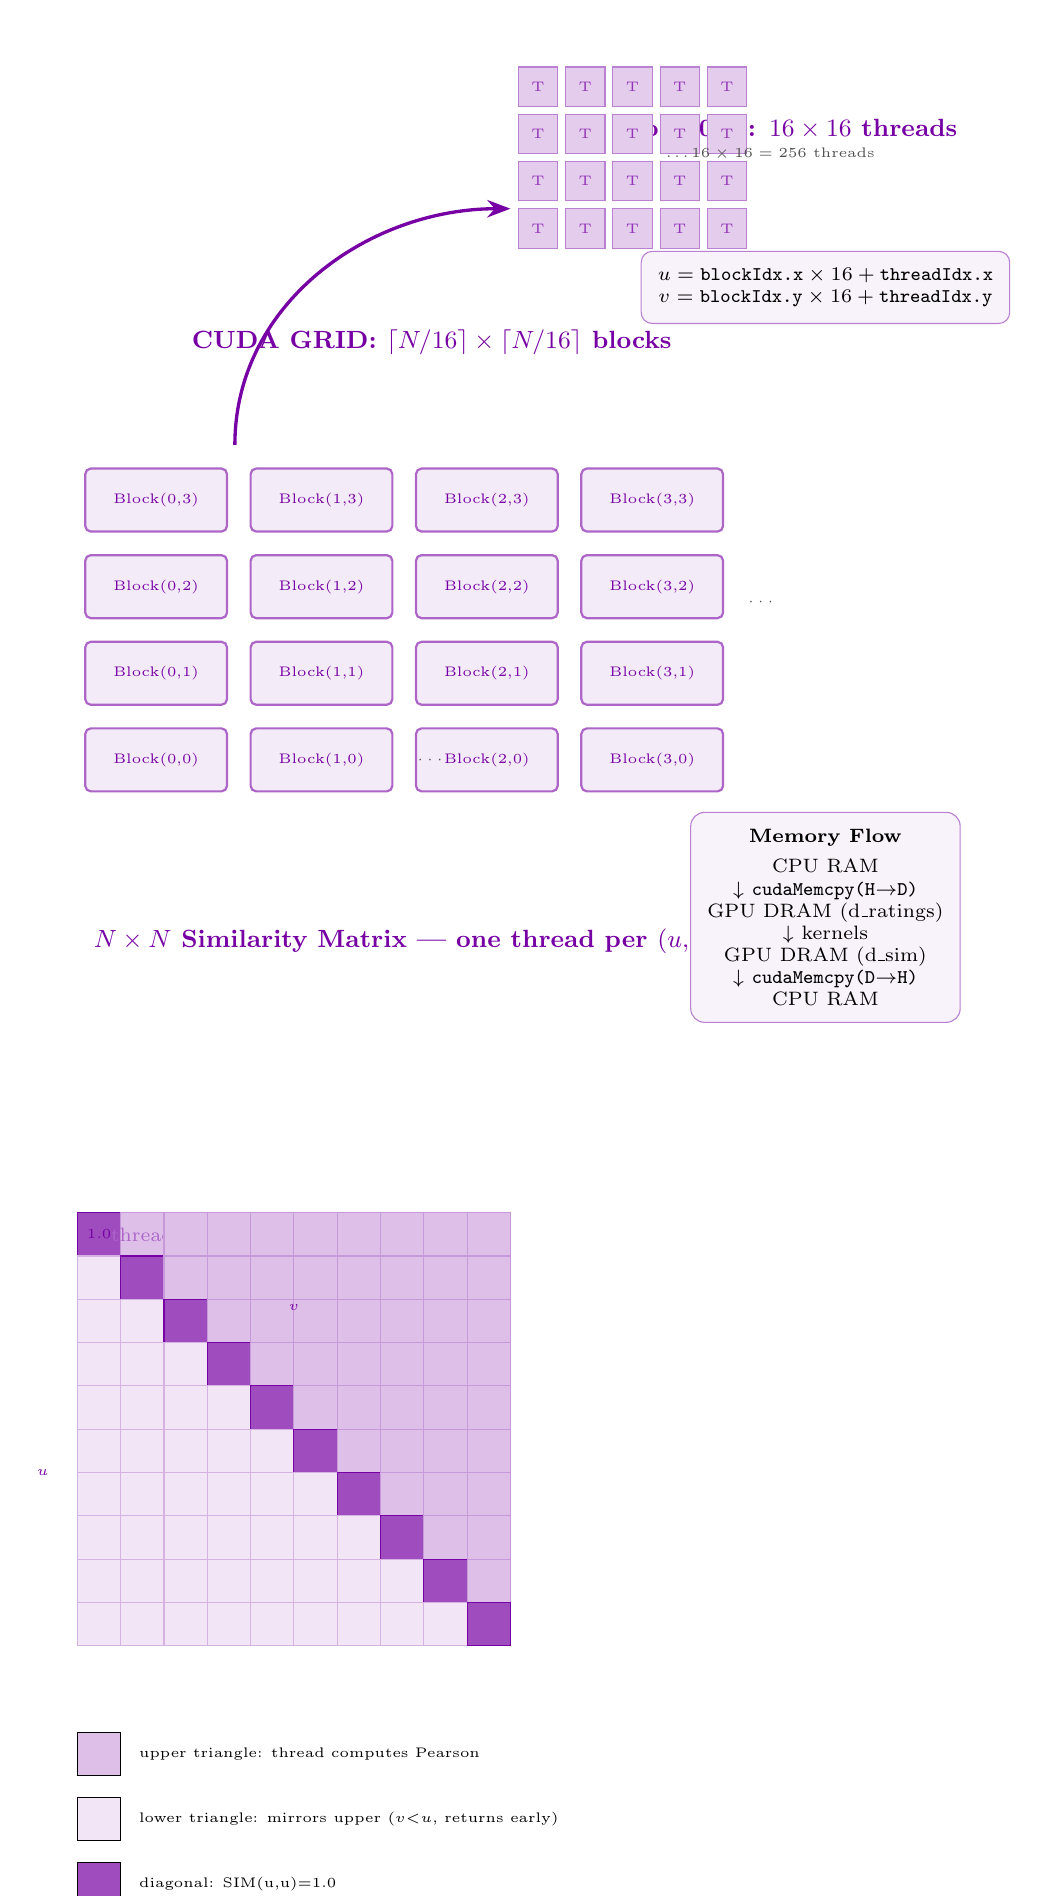
\begin{tikzpicture}[x=1cm,y=1cm]

% ── GRID label ────────────────────────────────────────────────────────────────
\node[font=\small\bfseries, cudacol] at (4.5,5.8)
      {CUDA GRID: $\lceil N/16 \rceil \times \lceil N/16 \rceil$ blocks};

% ── Draw grid of blocks ───────────────────────────────────────────────────────
\foreach \bx in {0,...,3} \foreach \by in {0,...,3} {
  \draw[cudacol!60, thick, fill=cudacol!8, rounded corners=2pt]
       (\bx*2.1+0.1, \by*1.1+0.1) rectangle (\bx*2.1+1.9, \by*1.1+0.9);
  \node[font=\tiny, cudacol] at (\bx*2.1+1.0, \by*1.1+0.5)
        {Block(\bx,\by)};
}
\node[font=\tiny, darkgray2] at (4.5,0.5) {$\cdots$};
\node[font=\tiny, darkgray2] at (8.7,2.5) {$\cdots$};

% ── Zoom into one block ───────────────────────────────────────────────────────
\draw[cudacol, very thick, -Stealth] (2.0,4.5) to[out=90,in=180] (5.5,7.5);

\node[font=\small\bfseries, cudacol] at (9,8.5) {Block(0,0): $16 \times 16$ threads};
\foreach \tx in {0,...,4} \foreach \ty in {0,...,3} {
  \draw[fill=cudacol!20, draw=cudacol!50]
       (5.6+\tx*0.6, 7.0+\ty*0.6) rectangle (6.1+\tx*0.6, 7.5+\ty*0.6);
  \node[font=\tiny\color{cudacol!80}] at (5.85+\tx*0.6, 7.25+\ty*0.6)
        {\tiny T};
}
\node[font=\tiny, darkgray2] at (8.8,8.2) {\ldots $16\times16=256$ threads};

% Thread index formula
\node[draw=cudacol!50, rounded corners, fill=cudacol!5, inner sep=6pt,
      font=\scriptsize] at (9.5,6.5) {
  $u = \texttt{blockIdx.x} \times 16 + \texttt{threadIdx.x}$\\
  $v = \texttt{blockIdx.y} \times 16 + \texttt{threadIdx.y}$
};

% ── Similarity matrix mapping ─────────────────────────────────────────────────
\node[font=\small\bfseries, cudacol] at (4.5,-1.8)
      {$N \times N$ Similarity Matrix — one thread per $(u,v)$ cell};

\begin{scope}[yshift=-5.8cm, xscale=0.55, yscale=0.55]
  \foreach \r in {0,...,9} \foreach \c in {0,...,9} {
    \ifnum\c=\r
      \draw[fill=cudacol!70, draw=cudacol] (\c,-\r) rectangle (\c+1,-\r+1);
    \else
      \ifnum\c>\r
        \draw[fill=cudacol!25, draw=cudacol!40] (\c,-\r) rectangle (\c+1,-\r+1);
        \node[font=\tiny\color{cudacol!60}] at (\c+0.5,-\r+0.5)
              {\ifnum\c=1\ifnum\r=0 \scriptsize thread\fi\fi};
      \else
        \draw[fill=cudacol!10, draw=cudacol!30] (\c,-\r) rectangle (\c+1,-\r+1);
      \fi
    \fi
  }
  % Diagonal label
  \node[font=\tiny, cudacol] at (0.5,0.5) {1.0};
  % Labels
  \node[font=\tiny\bfseries, cudacol] at (5,-1.2) {$v$};
  \node[font=\tiny\bfseries, cudacol] at (-0.8,-5) {$u$};
  % Legend
  \draw[fill=cudacol!25] (0,-12) rectangle (1,-11);
  \node[font=\tiny, anchor=west] at (1.2,-11.5) {upper triangle: thread computes Pearson};
  \draw[fill=cudacol!10] (0,-13.5) rectangle (1,-12.5);
  \node[font=\tiny, anchor=west] at (1.2,-13) {lower triangle: mirrors upper ($v{<}u$, returns early)};
  \draw[fill=cudacol!70] (0,-15) rectangle (1,-14);
  \node[font=\tiny, anchor=west] at (1.2,-14.5) {diagonal: SIM(u,u)=1.0};
\end{scope}

% Memory flow
\node[draw=cudacol!50, rounded corners=5pt, fill=cudacol!5, inner sep=6pt,
      font=\scriptsize, align=center] at (9.5,-1.5)
      {\textbf{Memory Flow}\\[3pt]
       CPU RAM\\$\downarrow$ \texttt{cudaMemcpy(H$\to$D)}\\
       GPU DRAM (d\_ratings)\\$\downarrow$ kernels\\
       GPU DRAM (d\_sim)\\$\downarrow$ \texttt{cudaMemcpy(D$\to$H)}\\
       CPU RAM};

\end{tikzpicture}
\end{center}

\begin{mdframed}[style=descbox]
\textbf{Description.}  The CUDA version maps each $(u,v)$ pair of the
similarity matrix to one GPU thread.  A 2-D grid of $\lceil N/16 \rceil
\times \lceil N/16 \rceil$ blocks, each containing $16 \times 16 = 256$
threads, is launched for \texttt{kernel\_similarity}.  Thread $(u,v)$ computes
Pearson correlation for that pair and writes both \texttt{SIM(u,v)} and
\texttt{SIM(v,u)} atomically (race-free because each $(u,v)$ pair is unique
to one thread).  Threads in the lower triangle ($v < u$) return immediately
to avoid redundant computation.  The prediction kernel (\texttt{kernel\_predictions})
uses a 2-D grid over $(u, \text{item})$ pairs and maintains an in-register
min-heap of size \texttt{TOP\_K=20} per thread (since \texttt{qsort} is
unavailable in device code).  Kernel execution time is measured precisely
with CUDA events (not CPU wall-clock timers, because kernel launches are
asynchronous).  Data is transferred between CPU RAM and GPU DRAM via
\texttt{cudaMemcpy} over the PCIe bus before and after computation.
\end{mdframed}

\newpage

% =============================================================================
\section{Hybrid MPI+OpenMP — Two-Level Parallelism}
% =============================================================================

\subsection*{Diagram 7 — Hybrid Architecture on a Multi-Node Cluster}

\begin{center}
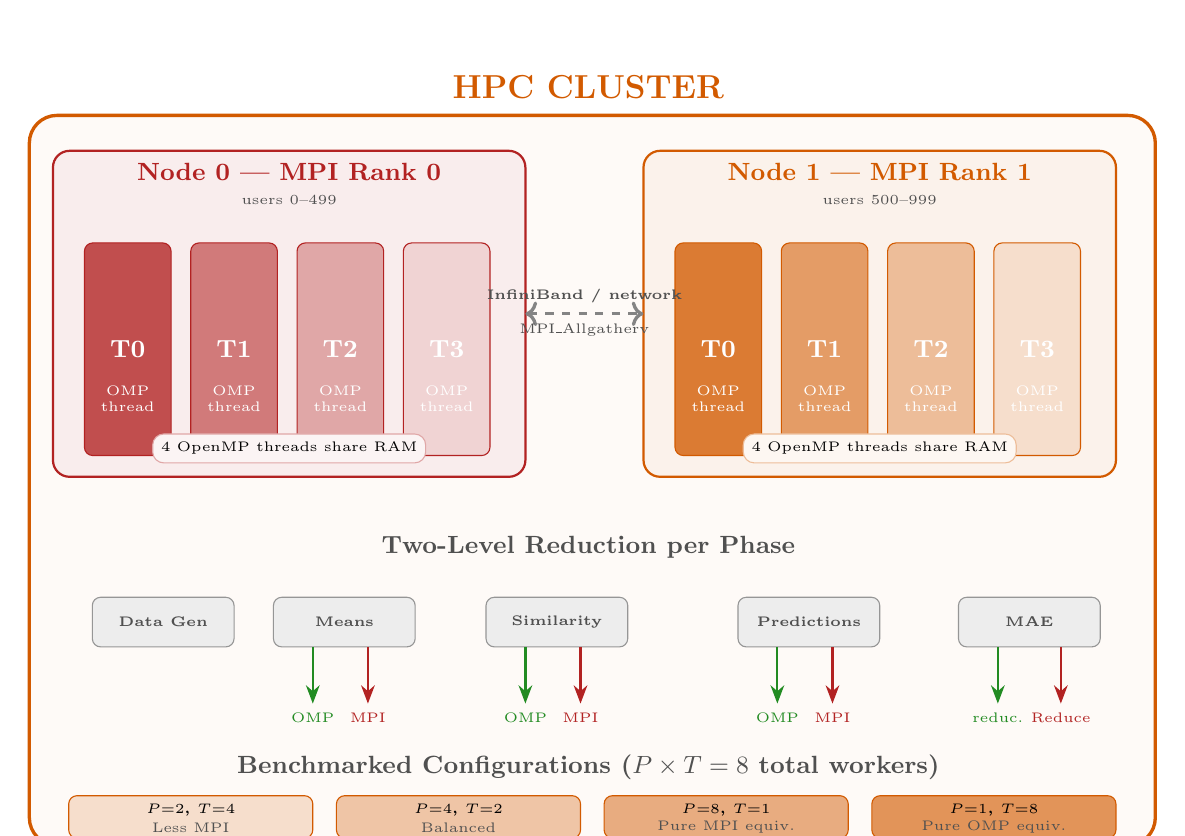
\begin{tikzpicture}[x=1cm,y=0.9cm]

% ── Cluster border ────────────────────────────────────────────────────────────
\draw[hybcol, very thick, rounded corners=10pt, fill=hybcol!3]
     (-0.3,-9.0) rectangle (14.0,1.3);
\node[font=\large\bfseries, hybcol] at (6.8,1.7) {HPC CLUSTER};

% ── Node 0 ────────────────────────────────────────────────────────────────────
\draw[mpicol, thick, rounded corners=6pt, fill=mpicol!8]
     (0.0,0.8) rectangle (6.0,-3.8);
\node[font=\small\bfseries, mpicol] at (3.0,0.5) {Node 0 — MPI Rank 0};
\node[font=\tiny, darkgray2] at (3.0,0.1) {users 0--499};

\foreach \t/\col in {0/mpicol!80, 1/mpicol!60, 2/mpicol!40, 3/mpicol!20} {
  \draw[fill=\col, draw=mpicol, rounded corners=3pt]
       (0.4+\t*1.35,-0.5) rectangle (1.5+\t*1.35,-3.5);
  \node[font=\small\bfseries, white] at (0.95+\t*1.35,-2.0)
        {T\t};
  \node[font=\tiny, white, align=center] at (0.95+\t*1.35,-2.7)
        {OMP\\ thread};
}
\node[draw=mpicol!40, rounded corners, fill=mpicol!5, font=\tiny,
      inner sep=3pt, align=center] at (3.0,-3.4)
      {4 OpenMP threads share RAM};

% ── Node 1 ────────────────────────────────────────────────────────────────────
\draw[hybcol, thick, rounded corners=6pt, fill=hybcol!8]
     (7.5,0.8) rectangle (13.5,-3.8);
\node[font=\small\bfseries, hybcol] at (10.5,0.5) {Node 1 — MPI Rank 1};
\node[font=\tiny, darkgray2] at (10.5,0.1) {users 500--999};

\foreach \t/\col in {0/hybcol!80, 1/hybcol!60, 2/hybcol!40, 3/hybcol!20} {
  \draw[fill=\col, draw=hybcol, rounded corners=3pt]
       (7.9+\t*1.35,-0.5) rectangle (9.0+\t*1.35,-3.5);
  \node[font=\small\bfseries, white] at (8.45+\t*1.35,-2.0) {T\t};
  \node[font=\tiny, white, align=center] at (8.45+\t*1.35,-2.7) {OMP\\ thread};
}
\node[draw=hybcol!40, rounded corners, fill=hybcol!5, font=\tiny,
      inner sep=3pt, align=center] at (10.5,-3.4)
      {4 OpenMP threads share RAM};

% ── InfiniBand link ──────────────────────────────────────────────────────────
\draw[very thick, dashed, darkgray2!70, <->] (6.0,-1.5) -- (7.5,-1.5)
      node[midway, above, font=\tiny\bfseries, darkgray2]{InfiniBand / network};
\node[font=\tiny, darkgray2, below] at (6.75,-1.5) {MPI\_Allgatherv};

% ── Phase timeline ────────────────────────────────────────────────────────────
\node[font=\small\bfseries, darkgray2] at (6.8,-4.8)
      {Two-Level Reduction per Phase};

\foreach \ph/\xpos/\lbl in {
    1/0.5/Data Gen,
    2/2.8/Means,
    3/5.5/Similarity,
    4/8.7/Predictions,
    5/11.5/MAE}
{
  \draw[fill=darkgray2!10, draw=darkgray2!60, rounded corners=3pt]
       (\xpos,-5.5) rectangle (\xpos+1.8,-6.2);
  \node[font=\tiny\bfseries, darkgray2] at (\xpos+0.9,-5.85) {\lbl};
}

% Parallel arrows for Phase 2-4
\foreach \xpos in {2.8, 5.5, 8.7} {
  % OMP arrow
  \draw[-Stealth, ompcol, thick] (\xpos+0.5,-6.2) -- (\xpos+0.5,-7.0);
  \node[font=\tiny, ompcol] at (\xpos+0.5,-7.2) {OMP};
  % MPI arrow
  \draw[-Stealth, mpicol, thick] (\xpos+1.2,-6.2) -- (\xpos+1.2,-7.0);
  \node[font=\tiny, mpicol] at (\xpos+1.2,-7.2) {MPI};
}
% MAE two-level
\draw[-Stealth, ompcol, thick] (12.0,-6.2) -- (12.0,-7.0);
\node[font=\tiny, ompcol] at (12.0,-7.2) {reduc.};
\draw[-Stealth, mpicol, thick] (12.8,-6.2) -- (12.8,-7.0);
\node[font=\tiny, mpicol] at (12.8,-7.2) {Reduce};

% ── Config table ─────────────────────────────────────────────────────────────
\node[font=\small\bfseries, darkgray2] at (6.8,-7.9)
      {Benchmarked Configurations ($P \times T = 8$ total workers)};
\foreach \c/\p/\t/\desc in {
    0/2/4/Less MPI,
    1/4/2/Balanced,
    2/8/1/Pure MPI equiv.,
    3/1/8/Pure OMP equiv.}
{
  \draw[fill=hybcol!\the\numexpr 20+\c*15\relax, draw=hybcol, rounded corners=3pt]
       (0.2+\c*3.4,-8.3) rectangle (3.3+\c*3.4,-8.9);
  \node[font=\tiny\bfseries] at (1.75+\c*3.4,-8.5)
        {$P{=}\p$, $T{=}\t$};
  \node[font=\tiny, darkgray2] at (1.75+\c*3.4,-8.75) {\desc};
}

\end{tikzpicture}
\end{center}

\begin{mdframed}[style=descbox]
\textbf{Description.}  The Hybrid version combines MPI and OpenMP to exploit
both levels of parallelism present in a real HPC cluster.  At the
\textbf{coarse level}, MPI partitions $N_{\text{users}}$ rows across $P$
ranks (processes), each running on a separate node with its own private RAM.
At the \textbf{fine level}, within each MPI rank, $T$ OpenMP threads
cooperate over the rank's row slice using shared memory, with no additional
MPI messages.  Total effective workers = $P \times T$, but MPI collectives
(\texttt{MPI\_Allgatherv}, \texttt{MPI\_Reduce}) involve only $P$ messages
— far fewer than a pure MPI program with $P \times T$ processes.
\texttt{MPI\_Init\_thread} with \texttt{MPI\_THREAD\_FUNNELED} is used
because MPI calls occur only from the main thread (outside
\texttt{\#pragma omp parallel} regions).  Phase~5 uses a two-level reduction:
OpenMP's \texttt{reduction(+:local\_err)} merges per-thread partial sums
within each rank, then \texttt{MPI\_Reduce} sums per-rank totals to rank~0.
Four configurations ($2{\times}4$, $4{\times}2$, $8{\times}1$, $1{\times}8$)
were benchmarked, all with 8 total workers, to reveal how different
MPI-to-OpenMP ratios affect performance.
\end{mdframed}

\newpage

% =============================================================================
\section{Summary: Parallel Concept Application Table}
% =============================================================================

\begin{center}
\renewcommand{\arraystretch}{1.4}
\begin{tabular}{>{\bfseries}p{2.3cm} p{2.5cm} p{2.8cm} p{3.5cm} p{2.8cm}}
\toprule
Version & Memory Model & Work Division & Synchronisation & Key API / Directive \\
\midrule
Serial &
  Shared (1 core) &
  None &
  None &
  \texttt{clock\_gettime} \\

\rowcolor{ompcol!10}
OpenMP &
  Shared (all threads) &
  \texttt{schedule(dynamic,4)} outer loop $u$ &
  Implicit barrier at \texttt{\}} &
  \texttt{\#pragma omp parallel for}, \texttt{reduction} \\

Pthreads &
  Shared (all threads) &
  Ceiling-division \texttt{work\_range()} &
  \texttt{pthread\_join} loop &
  \texttt{pthread\_create}, \texttt{pthread\_join} \\

\rowcolor{mpicol!8}
MPI &
  Distributed (private per rank) &
  Row blocks via \texttt{get\_range()} &
  \texttt{MPI\_Barrier} + collective ops &
  \texttt{MPI\_Allgatherv}, \texttt{MPI\_Reduce} \\

CUDA &
  Host + GPU DRAM &
  1 thread per $(u,v)$ or $(u,i)$ cell &
  \texttt{cudaDeviceSynchronize} &
  \texttt{\_\_global\_\_} kernels, \texttt{dim3} launch \\

\rowcolor{hybcol!8}
Hybrid &
  Distributed (MPI) + Shared (OMP) &
  MPI rows, OMP within rank &
  OMP barrier then MPI collective &
  \texttt{MPI\_Init\_thread}, \texttt{\#pragma omp} \\
\bottomrule
\end{tabular}
\end{center}

\vspace{1em}

% ── Final summary paragraph ───────────────────────────────────────────────────
\begin{mdframed}[style=descbox]
\textbf{Overall Parallelisation Strategy.}  The bottleneck phases (Similarity,
$O(N^2 M)$, and Predictions, $O(N^2 M)$) account for $>97\%$ of execution time.
All five parallel versions target these phases with the same algorithmic
approach — row-level work distribution — but differ in how they implement it:
shared memory (OpenMP, Pthreads) vs.\ distributed memory (MPI) vs.\ GPU
threads (CUDA) vs.\ a combination (Hybrid).  The serial fraction (fixed-seed
data generation) is kept in all versions to ensure numerical reproducibility:
every version produces the same \texttt{sim\_matrix} checksum and MAE
(within $\pm 0.001$), confirming correctness.  Speedup is measured as
$S(p) = T_{\text{serial}} / T_{\text{parallel}}(p)$ and efficiency as
$E(p) = S(p)/p$, benchmarked across thread/process counts of 1, 2, 4, and 8.
\end{mdframed}

\vfill
\begin{center}
\small\textit{Group 11 — EC7207/EE7218 High Performance Computing
  $\bullet$ Pearson Correlation Recommender System}
\end{center}

\end{document}
